% ============================================================================
% SECTION 2: DATABASE DESIGN
% ============================================================================
\section{Database Design}

\subsection{Entity-Relationship Diagram (Logical \& Physical ERD)}

The HistoryTalk persistence layer is built on \textbf{PostgreSQL 16} (relational schema \texttt{historical\_\ab schema}) integrated with \textbf{Supabase PgVector} (vector extension \texttt{vector(768)} with HNSW indexing). Schema evolution is strictly version-controlled through \textbf{Flyway Migrations (\texttt{V1} to \texttt{V38})}. Across all 6 bounded domains, the database comprises \textbf{32 tables} (30 JPA entity tables, 1 many-to-many join table \texttt{context\_\ab character\_\ab mapping}, and 1 vector store table \texttt{vector\_\ab chunk}).

\begin{figure}[htbp]
    \centering
    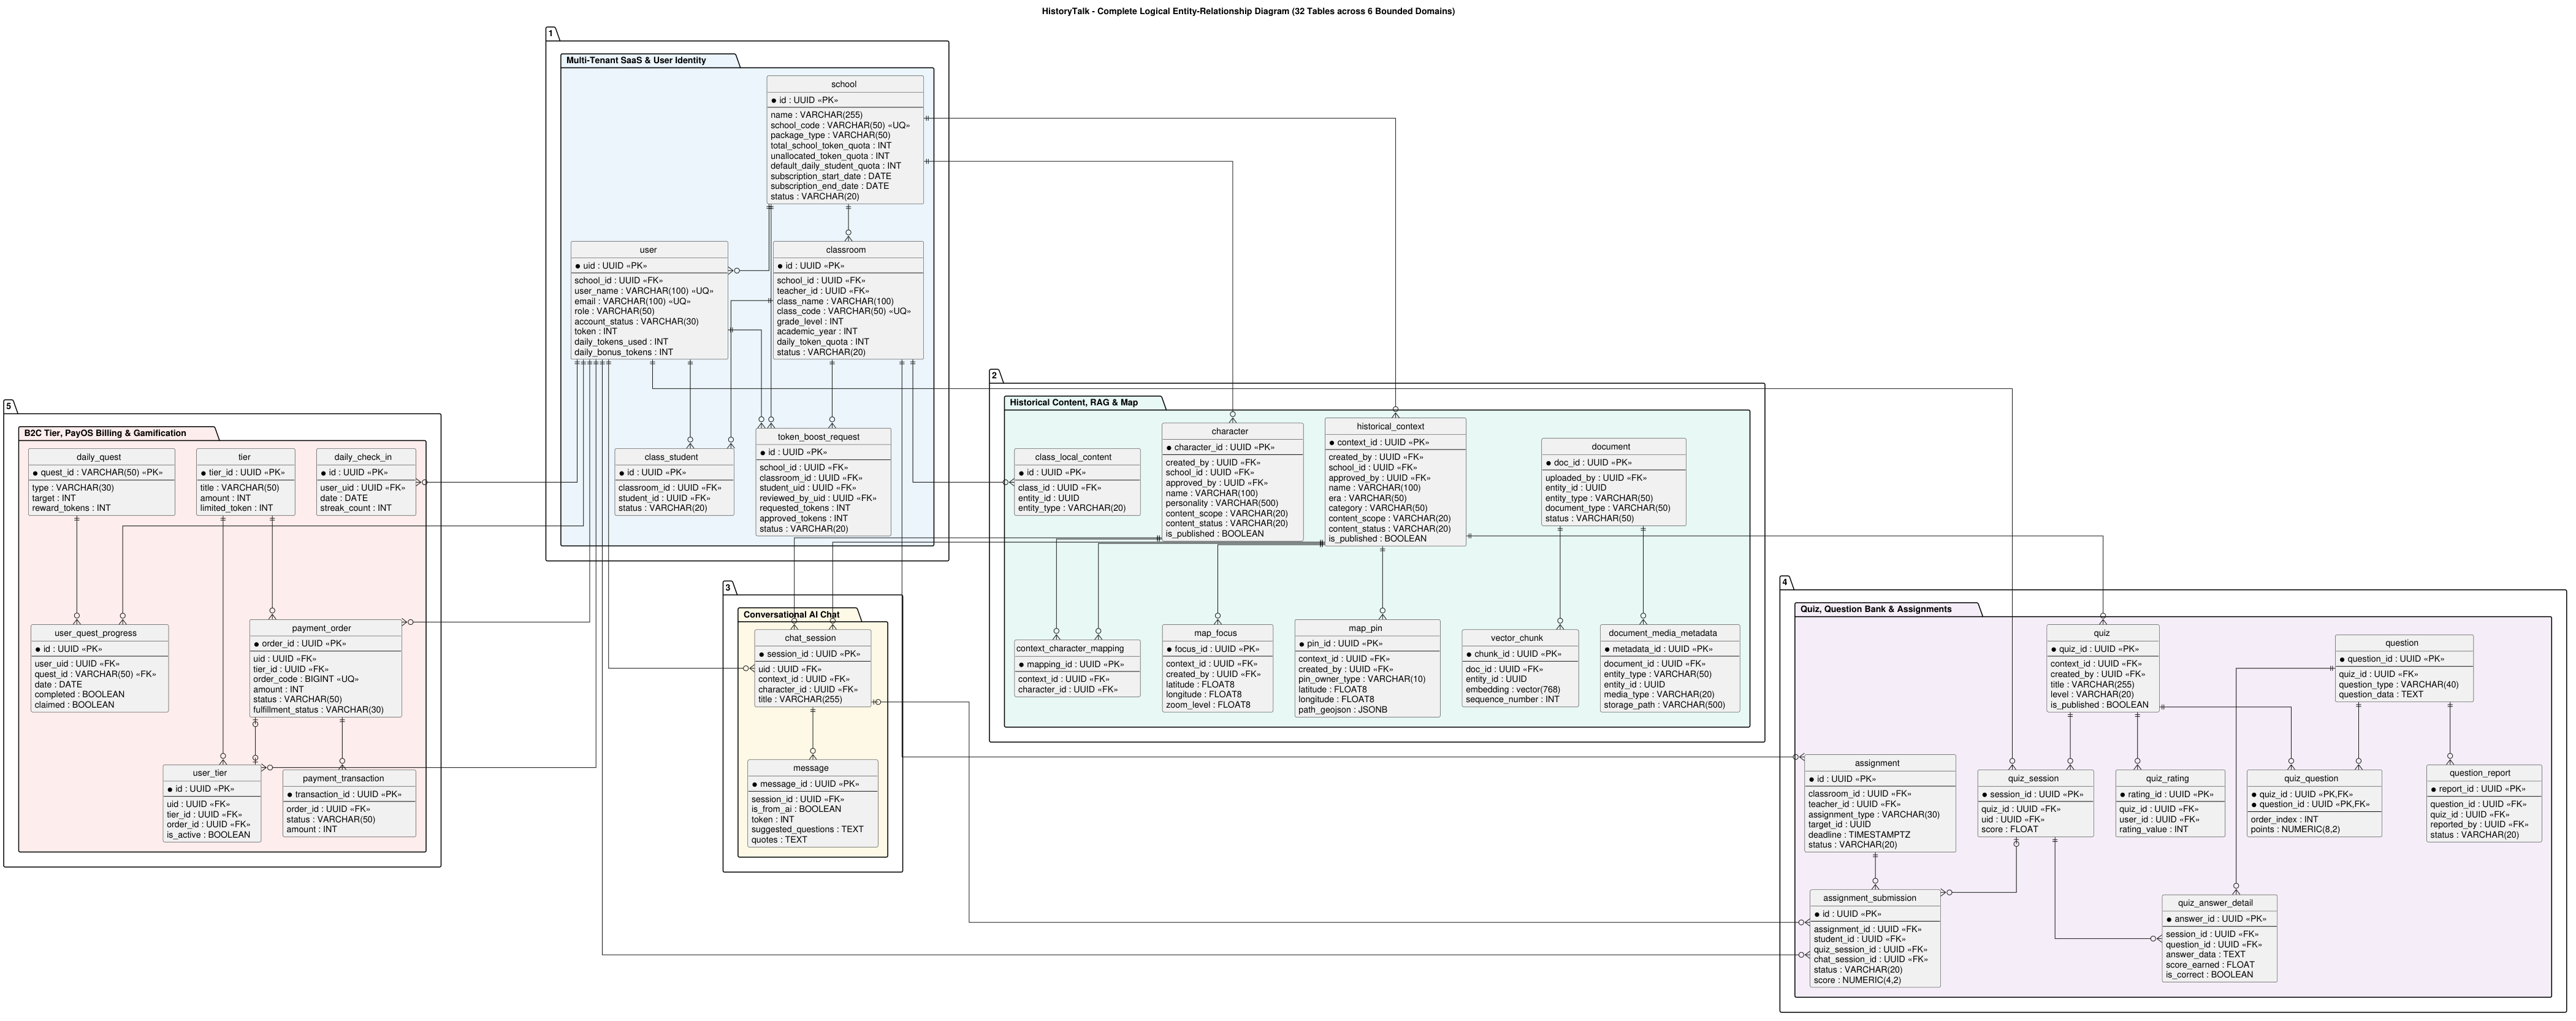
\includegraphics[width=0.99\textwidth,height=0.70\textheight,keepaspectratio]{figures/erd_full_overview.png}
    \caption{Complete Logical Entity-Relationship Diagram (32 Database Tables across 6 Bounded Domains)}
    \label{fig:erd_full_overview}
\end{figure}

\newpage
\subsection{Table Descriptions}

Table~\ref{tab:db_table_descriptions} summarizes all 32 database tables in HistoryTalk, specifying the business purpose, Primary Keys (PK), and Foreign Keys (FK) of each table in alignment with the database migration scripts and JPA entity models.

\begin{longtable}{|C{0.9cm}|L{4.2cm}|L{9.2cm}|}
\hline
\rowcolor{tableheader}
\textbf{No} & \textbf{Table} & \textbf{Description} \\
\hline
\endhead
01 & \texttt{school} & Stores B2B multi-tenant school organizations, enterprise subscription packages (\texttt{ENTERPRISE\_\ab SMALL}, \texttt{ENTERPRISE\_\ab MEDIUM}, \texttt{ENTERPRISE\_\ab LARGE}), shared token pools, academic subscription dates (\texttt{01/09}--\texttt{31/05}), and default daily student token quotas.\newline
$\bullet$ \textbf{Primary keys:} \texttt{id}\newline
$\bullet$ \textbf{Foreign keys:} None \\
\hline
02 & \texttt{"user"} & Stores all platform user accounts across 6 RBAC roles (\texttt{CUSTOMER}, \texttt{CONTENT\_\ab ADMIN}, \texttt{SYSTEM\_\ab ADMIN}, \texttt{SCHOOL\_\ab ADMIN}, \texttt{TEACHER}, \texttt{SCHOOL\_\ab STUDENT}), credentials, account status, B2C token balance, and B2B daily token consumption.\newline
$\bullet$ \textbf{Primary keys:} \texttt{uid}\newline
$\bullet$ \textbf{Foreign keys:} \texttt{school\_\ab id} $\rightarrow$ \texttt{school(id)} \\
\hline
03 & \texttt{classroom} & Represents school classrooms managed by teachers for a specific grade level (6--12) and academic year, with optional per-classroom daily token quota overrides.\newline
$\bullet$ \textbf{Primary keys:} \texttt{id}\newline
$\bullet$ \textbf{Foreign keys:} \texttt{school\_\ab id} $\rightarrow$ \texttt{school(id)}, \texttt{teacher\_\ab id} $\rightarrow$ \texttt{"user"(uid)} \\
\hline
04 & \texttt{class\_\ab student} & Junction table mapping enrolled school students to classrooms with enrollment timestamps and active status.\newline
$\bullet$ \textbf{Primary keys:} \texttt{id}\newline
$\bullet$ \textbf{Foreign keys:} \texttt{classroom\_\ab id} $\rightarrow$ \texttt{classroom(id)}, \texttt{student\_\ab id} $\rightarrow$ \texttt{"user"(uid)} \\
\hline
05 & \texttt{token\_\ab boost\_\ab request} & Tracks daily token boost requests submitted by school students when reaching their daily quota, and approval/rejection records by teachers or school admins.\newline
$\bullet$ \textbf{Primary keys:} \texttt{id}\newline
$\bullet$ \textbf{Foreign keys:} \texttt{school\_\ab id} $\rightarrow$ \texttt{school(id)}, \texttt{classroom\_\ab id} $\rightarrow$ \texttt{classroom(id)}, \texttt{student\_\ab uid} $\rightarrow$ \texttt{"user"(uid)}, \texttt{reviewed\_\ab by\_\ab uid} $\rightarrow$ \texttt{"user"(uid)} \\
\hline
06 & \texttt{historical\_\ab context} & Stores historical events, eras (\texttt{ANCIENT}, \texttt{MEDIEVAL}, \texttt{MODERN}, \texttt{CONTEMPORARY}), categories, GeoJSON battle-map overlays, and multi-tenant local content approval states.\newline
$\bullet$ \textbf{Primary keys:} \texttt{context\_\ab id}\newline
$\bullet$ \textbf{Foreign keys:} \texttt{created\_\ab by} $\rightarrow$ \texttt{"user"(uid)}, \texttt{school\_\ab id} $\rightarrow$ \texttt{school(id)}, \texttt{approved\_\ab by} $\rightarrow$ \texttt{"user"(uid)} \\
\hline
07 & \texttt{"character"} & Stores historical figure personas, biographical backgrounds, speaking styles/personalities, 2D avatars, 3D model URLs (\texttt{.glb}), lifespan dates, and local content approval states.\newline
$\bullet$ \textbf{Primary keys:} \texttt{character\_\ab id}\newline
$\bullet$ \textbf{Foreign keys:} \texttt{created\_\ab by} $\rightarrow$ \texttt{"user"(uid)}, \texttt{school\_\ab id} $\rightarrow$ \texttt{school(id)}, \texttt{approved\_\ab by} $\rightarrow$ \texttt{"user"(uid)} \\
\hline
08 & \texttt{context\_\ab character\_\ab mapping} & Many-to-many bridge table associating historical characters with one or more historical contexts/campaigns.\newline
$\bullet$ \textbf{Primary keys:} \texttt{mapping\_\ab id}\newline
$\bullet$ \textbf{Foreign keys:} \texttt{context\_\ab id} $\rightarrow$ \texttt{historical\_\ab context(context\_\ab id)}, \texttt{character\_\ab id} $\rightarrow$ \texttt{"character"(character\_\ab id)} \\
\hline
09 & \texttt{class\_\ab local\_\ab content} & Assigns school-owned local historical contexts or characters (\texttt{CLASS\_\ab ONLY} or \texttt{SCHOOL\_\ab WIDE}) to specific classrooms.\newline
$\bullet$ \textbf{Primary keys:} \texttt{id}\newline
$\bullet$ \textbf{Foreign keys:} \texttt{class\_\ab id} $\rightarrow$ \texttt{classroom(id)}, \texttt{assigned\_\ab by} $\rightarrow$ \texttt{"user"(uid)} \\
\hline
10 & \texttt{document} & Stores reference historical documents (\texttt{TEXT}, \texttt{MARKDOWN}, \texttt{PDF}, \texttt{IMAGE\_\ab 2D}, \texttt{IMAGE\_\ab 3D}) attached polymorphically to contexts or characters for RAG grounding.\newline
$\bullet$ \textbf{Primary keys:} \texttt{doc\_\ab id}\newline
$\bullet$ \textbf{Foreign keys:} \texttt{uploaded\_\ab by} $\rightarrow$ \texttt{"user"(uid)} \\
\hline
11 & \texttt{document\_\ab media\_\ab metadata} & Polymorphic media metadata table storing Cloudflare R2 / Supabase Storage paths, dimensions, file sizes, and formats for characters, contexts, documents, and avatars.\newline
$\bullet$ \textbf{Primary keys:} \texttt{metadata\_\ab id}\newline
$\bullet$ \textbf{Foreign keys:} \texttt{document\_\ab id} $\rightarrow$ \texttt{document(doc\_\ab id)} \\
\hline
12 & \texttt{vector\_\ab chunk} & Supabase PgVector table storing semantically chunked document passages and 768-dimensional \texttt{BAAI/bge-m3} embeddings indexed with HNSW cosine similarity.\newline
$\bullet$ \textbf{Primary keys:} \texttt{chunk\_\ab id}\newline
$\bullet$ \textbf{Foreign keys:} \texttt{doc\_\ab id} $\rightarrow$ \texttt{document(doc\_\ab id)} \\
\hline
13 & \texttt{map\_\ab pin} & Stores interactive map markers (\texttt{ADMIN} or \texttt{USER} owned), coordinates, historical years, and GeoJSON \texttt{LineString} troop movement paths for a historical context.\newline
$\bullet$ \textbf{Primary keys:} \texttt{pin\_\ab id}\newline
$\bullet$ \textbf{Foreign keys:} \texttt{context\_\ab id} $\rightarrow$ \texttt{historical\_\ab context(context\_\ab id)}, \texttt{created\_\ab by} $\rightarrow$ \texttt{"user"(uid)} \\
\hline
14 & \texttt{map\_\ab focus} & Stores predefined camera viewpoints (latitude, longitude, zoom level, display order) to guide learners through key geographical stages of a campaign.\newline
$\bullet$ \textbf{Primary keys:} \texttt{focus\_\ab id}\newline
$\bullet$ \textbf{Foreign keys:} \texttt{context\_\ab id} $\rightarrow$ \texttt{historical\_\ab context(context\_\ab id)}, \texttt{created\_\ab by} $\rightarrow$ \texttt{"user"(uid)} \\
\hline
15 & \texttt{chat\_\ab session} & Tracks conversational AI roleplay sessions between a user and a historical character within a specific historical context.\newline
$\bullet$ \textbf{Primary keys:} \texttt{session\_\ab id}\newline
$\bullet$ \textbf{Foreign keys:} \texttt{uid} $\rightarrow$ \texttt{"user"(uid)}, \texttt{context\_\ab id} $\rightarrow$ \texttt{historical\_\ab context(context\_\ab id)}, \texttt{character\_\ab id} $\rightarrow$ \texttt{"character"(character\_\ab id)} \\
\hline
16 & \texttt{message} & Stores individual user and AI dialogue turns within a chat session, including token usage, 3 AI-suggested follow-up questions, and cited RAG historical quotes.\newline
$\bullet$ \textbf{Primary keys:} \texttt{message\_\ab id}\newline
$\bullet$ \textbf{Foreign keys:} \texttt{session\_\ab id} $\rightarrow$ \texttt{chat\_\ab session(session\_\ab id)} \\
\hline
17 & \texttt{quiz} & Stores assessment quizzes linked to historical contexts, categorized by difficulty level (\texttt{EASY}, \texttt{MEDIUM}, \texttt{HARD}) and publication status.\newline
$\bullet$ \textbf{Primary keys:} \texttt{quiz\_\ab id}\newline
$\bullet$ \textbf{Foreign keys:} \texttt{context\_\ab id} $\rightarrow$ \texttt{historical\_\ab context(context\_\ab id)}, \texttt{created\_\ab by} $\rightarrow$ \texttt{"user"(uid)} \\
\hline
18 & \texttt{question} & Central question bank supporting three polymorphic question types (\texttt{MULTIPLE\_\ab CHOICE}, \texttt{FILL\_\ab IN\_\ab BLANK}, \texttt{MATCHING}) with JSON payload \texttt{question\_\ab data} and explanations.\newline
$\bullet$ \textbf{Primary keys:} \texttt{question\_\ab id}\newline
$\bullet$ \textbf{Foreign keys:} \texttt{quiz\_\ab id} $\rightarrow$ \texttt{quiz(quiz\_\ab id)} (nullable for bank questions) \\
\hline
19 & \texttt{quiz\_\ab question} & Many-to-many link table binding reusable Question Bank items to Quizzes with explicit \texttt{order\_\ab index} and point weights (\texttt{points}).\newline
$\bullet$ \textbf{Primary keys:} \texttt{(quiz\_\ab id, question\_\ab id)}\newline
$\bullet$ \textbf{Foreign keys:} \texttt{quiz\_\ab id} $\rightarrow$ \texttt{quiz(quiz\_\ab id)}, \texttt{question\_\ab id} $\rightarrow$ \texttt{question(question\_\ab id)} \\
\hline
20 & \texttt{quiz\_\ab session} & Records a learner's timed quiz attempt, start/end timestamps, time limit, and final calculated score on a 10-point scale.\newline
$\bullet$ \textbf{Primary keys:} \texttt{session\_\ab id}\newline
$\bullet$ \textbf{Foreign keys:} \texttt{quiz\_\ab id} $\rightarrow$ \texttt{quiz(quiz\_\ab id)}, \texttt{uid} $\rightarrow$ \texttt{"user"(uid)} \\
\hline
21 & \texttt{quiz\_\ab answer\_\ab detail} & Stores per-question submitted answer JSON (\texttt{answer\_\ab data}), correctness flag, and points earned within a quiz attempt session.\newline
$\bullet$ \textbf{Primary keys:} \texttt{answer\_\ab id}\newline
$\bullet$ \textbf{Foreign keys:} \texttt{session\_\ab id} $\rightarrow$ \texttt{quiz\_\ab session(session\_\ab id)}, \texttt{question\_\ab id} $\rightarrow$ \texttt{question(question\_\ab id)} \\
\hline
22 & \texttt{quiz\_\ab rating} & Stores 1--5 star ratings submitted by learners after completing a quiz (enforcing one rating per user per quiz).\newline
$\bullet$ \textbf{Primary keys:} \texttt{rating\_\ab id}\newline
$\bullet$ \textbf{Foreign keys:} \texttt{quiz\_\ab id} $\rightarrow$ \texttt{quiz(quiz\_\ab id)}, \texttt{user\_\ab id} $\rightarrow$ \texttt{"user"(uid)} \\
\hline
23 & \texttt{question\_\ab report} & Stores learner/teacher error reports flagging factual or formatting issues on specific quiz questions for Content Admin review.\newline
$\bullet$ \textbf{Primary keys:} \texttt{report\_\ab id}\newline
$\bullet$ \textbf{Foreign keys:} \texttt{question\_\ab id} $\rightarrow$ \texttt{question(question\_\ab id)}, \texttt{quiz\_\ab id} $\rightarrow$ \texttt{quiz(quiz\_\ab id)}, \texttt{reported\_\ab by} $\rightarrow$ \texttt{"user"(uid)} \\
\hline
24 & \texttt{assignment} & Stores classroom homework assignments created by teachers across three learning modes (\texttt{CONTEXT\_\ab READING}, \texttt{AI\_\ab CHAT\_\ab ROLEPLAY}, \texttt{QUIZ\_\ab TEST}) with deadlines and minimum completion thresholds.\newline
$\bullet$ \textbf{Primary keys:} \texttt{id}\newline
$\bullet$ \textbf{Foreign keys:} \texttt{classroom\_\ab id} $\rightarrow$ \texttt{classroom(id)}, \texttt{teacher\_\ab id} $\rightarrow$ \texttt{"user"(uid)} \\
\hline
25 & \texttt{assignment\_\ab submission} & Tracks individual student progress, submission status (\texttt{NOT\_\ab STARTED}, \texttt{IN\_\ab PROGRESS}, \texttt{SUBMITTED}, \texttt{LATE\_\ab SUBMITTED}, \texttt{MISSED}, \texttt{EXEMPTED}), score, AI chat message count, and reading duration.\newline
$\bullet$ \textbf{Primary keys:} \texttt{id}\newline
$\bullet$ \textbf{Foreign keys:} \texttt{assignment\_\ab id} $\rightarrow$ \texttt{assignment(id)}, \texttt{student\_\ab id} $\rightarrow$ \texttt{"user"(uid)}, \texttt{quiz\_\ab session\_\ab id} $\rightarrow$ \texttt{quiz\_\ab session(session\_\ab id)}, \texttt{chat\_\ab session\_\ab id} $\rightarrow$ \texttt{chat\_\ab session(session\_\ab id)} \\
\hline
26 & \texttt{tier} & Defines B2C subscription plans (e.g., Free, Plus, Pro), pricing in VND, billing duration in months, and token allowances.\newline
$\bullet$ \textbf{Primary keys:} \texttt{tier\_\ab id}\newline
$\bullet$ \textbf{Foreign keys:} None \\
\hline
27 & \texttt{user\_\ab tier} & Records active and historical B2C tier subscriptions for users, linking to the originating \texttt{payment\_\ab order}.\newline
$\bullet$ \textbf{Primary keys:} \texttt{id}\newline
$\bullet$ \textbf{Foreign keys:} \texttt{uid} $\rightarrow$ \texttt{"user"(uid)}, \texttt{tier\_\ab id} $\rightarrow$ \texttt{tier(tier\_\ab id)}, \texttt{order\_\ab id} $\rightarrow$ \texttt{payment\_\ab order(order\_\ab id)} \\
\hline
28 & \texttt{payment\_\ab order} & Tracks PayOS checkout orders, unique numeric \texttt{order\_\ab code}, QR checkout URLs, payment status (\texttt{PENDING}, \texttt{PAID}, \texttt{CANCELLED}, \texttt{EXPIRED}, \texttt{FAILED}), and resilient fulfillment state (\texttt{PENDING}, \texttt{PROCESSING}, \texttt{FULFILLED}, \texttt{FAILED}).\newline
$\bullet$ \textbf{Primary keys:} \texttt{order\_\ab id}\newline
$\bullet$ \textbf{Foreign keys:} \texttt{uid} $\rightarrow$ \texttt{"user"(uid)}, \texttt{tier\_\ab id} $\rightarrow$ \texttt{tier(tier\_\ab id)} \\
\hline
29 & \texttt{payment\_\ab transaction} & Immutable audit log of incoming PayOS webhook payloads, bank reference numbers, and verification statuses.\newline
$\bullet$ \textbf{Primary keys:} \texttt{transaction\_\ab id}\newline
$\bullet$ \textbf{Foreign keys:} \texttt{order\_\ab id} $\rightarrow$ \texttt{payment\_\ab order(order\_\ab id)} \\
\hline
30 & \texttt{daily\_\ab quest} & Master catalog of daily gamification quests (\texttt{CHAT}, \texttt{QUIZ}, \texttt{READ\_\ab CONTEXT}), completion targets, and token rewards.\newline
$\bullet$ \textbf{Primary keys:} \texttt{quest\_\ab id}\newline
$\bullet$ \textbf{Foreign keys:} None \\
\hline
31 & \texttt{user\_\ab quest\_\ab progress} & Tracks daily per-user progress toward active quests and reward claim status.\newline
$\bullet$ \textbf{Primary keys:} \texttt{id}\newline
$\bullet$ \textbf{Foreign keys:} \texttt{user\_\ab uid} $\rightarrow$ \texttt{"user"(uid)}, \texttt{quest\_\ab id} $\rightarrow$ \texttt{daily\_\ab quest(quest\_\ab id)} \\
\hline
32 & \texttt{daily\_\ab check\_\ab in} & Records daily user login check-ins and consecutive day streak counts.\newline
$\bullet$ \textbf{Primary keys:} \texttt{id}\newline
$\bullet$ \textbf{Foreign keys:} \texttt{user\_\ab uid} $\rightarrow$ \texttt{"user"(uid)} \\
\hline
\caption{Database Table Descriptions (32 Tables in \texttt{historical\_\ab schema} \& Supabase PgVector)}
\label{tab:db_table_descriptions}
\end{longtable}

\newpage
\subsection{Detailed Data Dictionary}

Table~\ref{tab:data_dictionary} provides the complete column-level specification for all 32 tables, synchronized with the Java JPA entity annotations and Flyway migrations \texttt{V1}--\texttt{V38}.

\footnotesize
\begin{longtable}{|L{3.8cm}|L{2.5cm}|L{2.1cm}|L{5.9cm}|}
\hline
\rowcolor{tableheader}
\textbf{Column Name} & \textbf{Data Type} & \textbf{Constraints} & \textbf{Description} \\
\hline
\endhead

\multicolumn{4}{|l|}{\cellcolor{lightgray}\textbf{Table 01: \texttt{school} -- B2B Multi-Tenant Partner Schools}} \\
\hline
\texttt{id} & \texttt{UUID} & \texttt{PK, NOT NULL} & Unique school tenant identifier. \\
\hline
\texttt{name} & \texttt{VARCHAR(255)} & \texttt{NOT NULL} & Official school name. \\
\hline
\texttt{school\_\ab code} & \texttt{VARCHAR(50)} & \texttt{UQ, NOT NULL} & Unique institutional code (e.g., \texttt{THPT-LHP-HCM}). \\
\hline
\texttt{address} & \texttt{VARCHAR(500)} & \texttt{NULLABLE} & Physical address of the school. \\
\hline
\texttt{contact\_\ab email} & \texttt{VARCHAR(100)} & \texttt{NOT NULL} & Primary administrative contact email. \\
\hline
\texttt{contact\_\ab phone} & \texttt{VARCHAR(20)} & \texttt{NULLABLE} & Contact phone number. \\
\hline
\texttt{package\_\ab type} & \texttt{VARCHAR(50)} & \texttt{NOT NULL} & Enum \texttt{EnterprisePackage}: \texttt{ENTERPRISE\_\ab SMALL} (5M), \texttt{ENTERPRISE\_\ab MEDIUM} (20M), \texttt{ENTERPRISE\_\ab LARGE} (50M). \\
\hline
\texttt{total\_\ab school\_\ab token\_\ab quota} & \texttt{INTEGER} & \texttt{NOT NULL} & Total contracted AI tokens for the academic year. \\
\hline
\texttt{unallocated\_\ab token\_\ab quota} & \texttt{INTEGER} & \texttt{NOT NULL} & Remaining shared token pool available for daily student consumption and boosts. \\
\hline
\texttt{subscription\_\ab start\_\ab date} & \texttt{DATE} & \texttt{NULLABLE} & Academic year start date (standard \texttt{01/09}). \\
\hline
\texttt{subscription\_\ab end\_\ab date} & \texttt{DATE} & \texttt{NULLABLE} & Academic year end date (standard \texttt{31/05}). \\
\hline
\texttt{renewed\_\ab for\_\ab next\_\ab year} & \texttt{BOOLEAN} & \texttt{DEFAULT FALSE} & Flag indicating pre-renewal for the next academic year. \\
\hline
\texttt{next\_\ab package\_\ab type} & \texttt{VARCHAR(50)} & \texttt{NULLABLE} & Next year's \texttt{EnterprisePackage} tier if pre-renewed. \\
\hline
\texttt{default\_\ab daily\_\ab student\_\ab quota} & \texttt{INTEGER} & \texttt{DEFAULT 1000} & Default daily AI token allowance per student. \\
\hline
\texttt{local\_\ab history\_\ab policy\_\ab accepted} & \texttt{BOOLEAN} & \texttt{DEFAULT FALSE} & Whether the School Admin accepted the Local History Content Policy. \\
\hline
\texttt{status} & \texttt{VARCHAR(20)} & \texttt{NOT NULL} & Enum \texttt{SchoolStatus}: \texttt{ACTIVE}, \texttt{INACTIVE}, \texttt{SUSPENDED}, \texttt{EXPIRED}. \\
\hline
\texttt{created\_\ab at / updated\_\ab at / deleted\_\ab at} & \texttt{TIMESTAMP} & \texttt{AUDIT} & Creation, modification, and soft-delete timestamps. \\
\hline

\multicolumn{4}{|l|}{\cellcolor{lightgray}\textbf{Table 02: \texttt{"user"} -- Platform User Accounts \& Multi-Tenant RBAC}} \\
\hline
\texttt{uid} & \texttt{UUID} & \texttt{PK, NOT NULL} & Unique user UUID. \\
\hline
\texttt{user\_\ab name} & \texttt{VARCHAR(100)} & \texttt{UQ, NOT NULL} & Unique login username. \\
\hline
\texttt{email} & \texttt{VARCHAR(100)} & \texttt{UQ, NOT NULL} & Unique login and notification email address. \\
\hline
\texttt{password} & \texttt{VARCHAR(100)} & \texttt{NOT NULL} & BCrypt-hashed password string. \\
\hline
\texttt{full\_\ab name} & \texttt{VARCHAR(150)} & \texttt{NULLABLE} & Full display name of the user. \\
\hline
\texttt{dob / gender / phone\_\ab number} & \texttt{DATE / VARCHAR} & \texttt{NULLABLE} & Date of birth, \texttt{Gender} (\texttt{MALE}, \texttt{FEMALE}, \texttt{OTHER}), and phone. \\
\hline
\texttt{address / avatar\_\ab url} & \texttt{VARCHAR(500)} & \texttt{NULLABLE} & Residential address and profile avatar URL. \\
\hline
\texttt{role} & \texttt{VARCHAR(50)} & \texttt{NOT NULL} & Enum \texttt{UserRole}: \texttt{CUSTOMER}, \texttt{CONTENT\_\ab ADMIN}, \texttt{SYSTEM\_\ab ADMIN}, \texttt{SCHOOL\_\ab ADMIN}, \texttt{TEACHER}, \texttt{SCHOOL\_\ab STUDENT}. \\
\hline
\texttt{school\_\ab id} & \texttt{UUID} & \texttt{FK, NULLABLE} & References \texttt{school(id)} for B2B institutional users. \\
\hline
\texttt{student\_\ab code} & \texttt{VARCHAR(50)} & \texttt{NULLABLE} & Institutional student code within the school. \\
\hline
\texttt{must\_\ab change\_\ab password} & \texttt{BOOLEAN} & \texttt{DEFAULT FALSE} & Forces password update on first login for CSV-imported accounts. \\
\hline
\texttt{subject\_\ab department} & \texttt{VARCHAR(100)} & \texttt{NULLABLE} & Academic department for \texttt{TEACHER} accounts. \\
\hline
\texttt{account\_\ab status} & \texttt{VARCHAR(30)} & \texttt{NOT NULL} & Enum \texttt{AccountStatus}: \texttt{ACTIVE}, \texttt{DEACTIVATED}. \\
\hline
\texttt{deactivated\_\ab reason} & \texttt{VARCHAR(255)} & \texttt{NULLABLE} & Audit reason for account deactivation (e.g., Grade 12 graduation). \\
\hline
\texttt{token} & \texttt{INTEGER} & \texttt{DEFAULT 0} & B2C customer token balance. \\
\hline
\texttt{daily\_\ab tokens\_\ab used} & \texttt{INTEGER} & \texttt{DEFAULT 0} & Tokens consumed today by a \texttt{SCHOOL\_\ab STUDENT}. \\
\hline
\texttt{daily\_\ab bonus\_\ab tokens} & \texttt{INTEGER} & \texttt{DEFAULT 0} & Approved boost tokens granted for the current day. \\
\hline
\texttt{last\_\ab active\_\ab date / last\_\ab token\_\ab reset\_\ab at} & \texttt{TIMESTAMP} & \texttt{NULLABLE} & Last activity and lazy daily token reset / JWT revocation timestamp. \\
\hline
\texttt{password\_\ab reset\_\ab token\_\ab hash / expires\_\ab at} & \texttt{VARCHAR(64) / TS} & \texttt{NULLABLE} & SHA-256 hash and expiry of active password reset token. \\
\hline
\texttt{created\_\ab at / updated\_\ab at / deleted\_\ab at} & \texttt{TIMESTAMP} & \texttt{AUDIT} & Standard lifecycle timestamps. \\
\hline

\multicolumn{4}{|l|}{\cellcolor{lightgray}\textbf{Table 03: \texttt{classroom} -- School Classrooms}} \\
\hline
\texttt{id} & \texttt{UUID} & \texttt{PK, NOT NULL} & Unique classroom identifier. \\
\hline
\texttt{school\_\ab id} & \texttt{UUID} & \texttt{FK, NOT NULL} & References \texttt{school(id)}. \\
\hline
\texttt{teacher\_\ab id} & \texttt{UUID} & \texttt{FK, NULLABLE} & References homeroom/history teacher \texttt{"user"(uid)}. \\
\hline
\texttt{class\_\ab name} & \texttt{VARCHAR(100)} & \texttt{NOT NULL} & Display name (e.g., \texttt{10A1}, \texttt{12C3}). \\
\hline
\texttt{class\_\ab code} & \texttt{VARCHAR(50)} & \texttt{UQ, NOT NULL} & Globally unique smart join code generated by \texttt{SmartClassCodeGenerator}. \\
\hline
\texttt{grade\_\ab level} & \texttt{INTEGER} & \texttt{NULLABLE} & Grade level (6 to 12). \\
\hline
\texttt{academic\_\ab year} & \texttt{INTEGER} & \texttt{NOT NULL} & Academic start year (e.g., \texttt{2026}). \\
\hline
\texttt{description} & \texttt{VARCHAR(500)} & \texttt{NULLABLE} & Classroom curriculum description. \\
\hline
\texttt{daily\_\ab token\_\ab quota} & \texttt{INTEGER} & \texttt{NULLABLE} & Optional classroom-specific daily student token limit override. \\
\hline
\texttt{status} & \texttt{VARCHAR(20)} & \texttt{DEFAULT 'ACTIVE'} & Classroom lifecycle state (\texttt{ACTIVE}, \texttt{ARCHIVED}). \\
\hline
\texttt{created\_\ab at / updated\_\ab at / deleted\_\ab at} & \texttt{TIMESTAMP} & \texttt{AUDIT} & Standard lifecycle timestamps. \\
\hline

\multicolumn{4}{|l|}{\cellcolor{lightgray}\textbf{Table 04: \texttt{class\_\ab student} -- Classroom Student Roster Association}} \\
\hline
\texttt{id} & \texttt{UUID} & \texttt{PK, NOT NULL} & Unique enrollment record ID. \\
\hline
\texttt{classroom\_\ab id} & \texttt{UUID} & \texttt{FK, NOT NULL} & References \texttt{classroom(id)}. \\
\hline
\texttt{student\_\ab id} & \texttt{UUID} & \texttt{FK, NOT NULL} & References \texttt{"user"(uid)} (Unique together with \texttt{classroom\_\ab id}). \\
\hline
\texttt{joined\_\ab at} & \texttt{TIMESTAMP} & \texttt{NOT NULL} & Enrollment timestamp. \\
\hline
\texttt{status} & \texttt{VARCHAR(20)} & \texttt{DEFAULT 'ACTIVE'} & Enrollment status (\texttt{ACTIVE}, \texttt{TRANSFERRED}, \texttt{REMOVED}). \\
\hline

\multicolumn{4}{|l|}{\cellcolor{lightgray}\textbf{Table 05: \texttt{token\_\ab boost\_\ab request} -- Student Daily Token Boost Workflow}} \\
\hline
\texttt{id} & \texttt{UUID} & \texttt{PK, NOT NULL} & Unique boost request ID. \\
\hline
\texttt{school\_\ab id / classroom\_\ab id} & \texttt{UUID} & \texttt{FK, NOT NULL} & References \texttt{school(id)} and \texttt{classroom(id)}. \\
\hline
\texttt{student\_\ab uid} & \texttt{UUID} & \texttt{FK, NOT NULL} & Requesting student \texttt{"user"(uid)}. \\
\hline
\texttt{requested\_\ab tokens / approved\_\ab tokens} & \texttt{INTEGER} & \texttt{NOT NULL / NULL} & Requested vs. approved bonus token count. \\
\hline
\texttt{reason / review\_\ab note} & \texttt{VARCHAR(500)} & \texttt{NOT NULL / NULL} & Student justification and teacher/admin review note. \\
\hline
\texttt{status} & \texttt{VARCHAR(20)} & \texttt{NOT NULL} & Enum \texttt{TokenBoostRequestStatus}: \texttt{PENDING}, \texttt{APPROVED}, \texttt{REJECTED}. \\
\hline
\texttt{reviewed\_\ab by\_\ab uid} & \texttt{UUID} & \texttt{FK, NULLABLE} & Teacher or School Admin \texttt{"user"(uid)} who reviewed the request. \\
\hline
\texttt{request\_\ab date / created\_\ab at / updated\_\ab at} & \texttt{DATE / TS} & \texttt{NOT NULL} & Request date and audit timestamps. \\
\hline

\multicolumn{4}{|l|}{\cellcolor{lightgray}\textbf{Table 06: \texttt{historical\_\ab context} -- Historical Events, Battles \& Local Content}} \\
\hline
\texttt{context\_\ab id} & \texttt{UUID} & \texttt{PK, NOT NULL} & Unique historical context UUID. \\
\hline
\texttt{name} & \texttt{VARCHAR(100)} & \texttt{UQ, NOT NULL} & Event/campaign title. \\
\hline
\texttt{description} & \texttt{TEXT} & \texttt{NOT NULL} & Detailed historical narrative and background. \\
\hline
\texttt{era} & \texttt{VARCHAR(30)} & \texttt{NULLABLE} & Enum \texttt{EventEra}: \texttt{ANCIENT}, \texttt{MEDIEVAL}, \texttt{MODERN}, \texttt{CONTEMPORARY}. \\
\hline
\texttt{category} & \texttt{VARCHAR(30)} & \texttt{NULLABLE} & Enum \texttt{EventCategory}: \texttt{WAR}, \texttt{POLITICS}, \texttt{CULTURE}, \texttt{SCIENCE}, \texttt{RELIGION}, \texttt{OTHER}. \\
\hline
\texttt{year / start\_\ab year / end\_\ab year / is\_\ab bc} & \texttt{INT / BOOLEAN} & \texttt{NULLABLE} & Chronological timeline indicators and Before Christ (\texttt{is\_\ab bc}) flag. \\
\hline
\texttt{location / latitude / longitude} & \texttt{VARCHAR / FLOAT8} & \texttt{NULLABLE} & Geographical location name and coordinates. \\
\hline
\texttt{image\_\ab url / video\_\ab url} & \texttt{VARCHAR(500)} & \texttt{NULLABLE} & Cover illustration and video media URLs. \\
\hline
\texttt{battle\_\ab map} & \texttt{JSONB} & \texttt{NULLABLE} & Interactive battle-map configuration JSON (factions, symbols, overlay). \\
\hline
\texttt{created\_\ab by / approved\_\ab by} & \texttt{UUID} & \texttt{FK} & Author \texttt{"user"(uid)} and approving School Admin \texttt{"user"(uid)}. \\
\hline
\texttt{school\_\ab id} & \texttt{UUID} & \texttt{FK, NULLABLE} & \texttt{NULL} for global content; \texttt{school(id)} for school-owned local content. \\
\hline
\texttt{content\_\ab scope} & \texttt{VARCHAR(20)} & \texttt{NULLABLE} & Enum \texttt{ContentScope}: \texttt{CLASS\_\ab ONLY}, \texttt{SCHOOL\_\ab WIDE}. \\
\hline
\texttt{content\_\ab status} & \texttt{VARCHAR(20)} & \texttt{NULLABLE} & Enum \texttt{ContentStatus}: \texttt{DRAFT}, \texttt{PENDING\_\ab REVIEW}, \texttt{ACTIVE}, \texttt{INACTIVE}. \\
\hline
\texttt{review\_\ab note / is\_\ab published} & \texttt{TEXT / BOOLEAN} & \texttt{NULL / DEFAULT F} & Admin review feedback note and public visibility flag. \\
\hline
\texttt{created\_\ab at / updated\_\ab at / deleted\_\ab at} & \texttt{TIMESTAMP} & \texttt{AUDIT} & Standard lifecycle timestamps. \\
\hline

\multicolumn{4}{|l|}{\cellcolor{lightgray}\textbf{Table 07: \texttt{"character"} -- Historical Character Personas}} \\
\hline
\texttt{character\_\ab id} & \texttt{UUID} & \texttt{PK, NOT NULL} & Unique character UUID. \\
\hline
\texttt{name / title} & \texttt{VARCHAR(100/150)} & \texttt{NOT NULL / NULL} & Character name and historical title/honorific. \\
\hline
\texttt{background} & \texttt{TEXT} & \texttt{NOT NULL} & Comprehensive biographical grounding text. \\
\hline
\texttt{personality} & \texttt{VARCHAR(500)} & \texttt{NULLABLE} & Persona tone, temperament, and speaking style prompt traits. \\
\hline
\texttt{image\_\ab url / character\_\ab model\_\ab url} & \texttt{VARCHAR(255/500)} & \texttt{NULLABLE} & 2D avatar URL and 3D \texttt{.glb} model URL. \\
\hline
\texttt{born\_\ab year/month/day / is\_\ab born\_\ab bc} & \texttt{INT / BOOLEAN} & \texttt{NULLABLE} & Structured birth date fields supporting BCE/CE eras. \\
\hline
\texttt{death\_\ab year/month/day / is\_\ab death\_\ab bc} & \texttt{INT / BOOLEAN} & \texttt{NULLABLE} & Structured death date fields supporting BCE/CE eras. \\
\hline
\texttt{created\_\ab by / school\_\ab id / approved\_\ab by} & \texttt{UUID} & \texttt{FK} & Creator, owning school (for local characters), and approver. \\
\hline
\texttt{content\_\ab scope / content\_\ab status} & \texttt{VARCHAR(20)} & \texttt{NULLABLE} & \texttt{ContentScope} and \texttt{ContentStatus} (\texttt{DRAFT}, \texttt{PENDING\_\ab REVIEW}, \texttt{ACTIVE}, \texttt{INACTIVE}). \\
\hline
\texttt{review\_\ab note / is\_\ab published} & \texttt{TEXT / BOOLEAN} & \texttt{NULL / DEFAULT F} & School Admin review note and publication status. \\
\hline
\texttt{created\_\ab at / updated\_\ab at / deleted\_\ab at} & \texttt{TIMESTAMP} & \texttt{AUDIT} & Standard lifecycle timestamps. \\
\hline

\multicolumn{4}{|l|}{\cellcolor{lightgray}\textbf{Table 08: \texttt{context\_\ab character\_\ab mapping} -- Context-Character M:N Join Table}} \\
\hline
\texttt{mapping\_\ab id} & \texttt{UUID} & \texttt{PK, NOT NULL} & Surrogate primary key. \\
\hline
\texttt{context\_\ab id / character\_\ab id} & \texttt{UUID} & \texttt{FK, UQ PAIR} & References \texttt{historical\_\ab context(context\_\ab id)} and \texttt{"character"(character\_\ab id)}. \\
\hline

\multicolumn{4}{|l|}{\cellcolor{lightgray}\textbf{Table 09: \texttt{class\_\ab local\_\ab content} -- Classroom Local Content Assignment}} \\
\hline
\texttt{id} & \texttt{UUID} & \texttt{PK, NOT NULL} & Unique assignment row ID. \\
\hline
\texttt{class\_\ab id} & \texttt{UUID} & \texttt{FK, NOT NULL} & Target \texttt{classroom(id)}. \\
\hline
\texttt{entity\_\ab id / entity\_\ab type} & \texttt{UUID / VARCHAR(20)} & \texttt{NOT NULL} & Polymorphic reference (\texttt{CONTEXT} or \texttt{CHARACTER}). \\
\hline
\texttt{assigned\_\ab by / assigned\_\ab at} & \texttt{UUID / TIMESTAMP} & \texttt{NULL / NOT NULL} & Teacher who assigned the content and timestamp. \\
\hline

\multicolumn{4}{|l|}{\cellcolor{lightgray}\textbf{Table 10: \texttt{document} -- RAG Historical Source Documents}} \\
\hline
\texttt{doc\_\ab id} & \texttt{UUID} & \texttt{PK, NOT NULL} & Unique document UUID. \\
\hline
\texttt{uploaded\_\ab by} & \texttt{UUID} & \texttt{FK, NOT NULL} & References uploader \texttt{"user"(uid)}. \\
\hline
\texttt{entity\_\ab id / entity\_\ab type} & \texttt{UUID / VARCHAR(20)} & \texttt{NOT NULL} & Polymorphic owner (\texttt{CONTEXT}, \texttt{CHARACTER}, \texttt{DOCUMENT}, \texttt{USER}). \\
\hline
\texttt{title / file\_\ab url} & \texttt{VARCHAR(255/500)} & \texttt{NOT NULL / NULL} & Document title and cloud storage file URL. \\
\hline
\texttt{content} & \texttt{TEXT} & \texttt{NULLABLE} & Extracted UTF-8 text (via PDFBox, Tess4J OCR, or Markdown). \\
\hline
\texttt{document\_\ab type} & \texttt{VARCHAR(20)} & \texttt{NOT NULL} & Enum \texttt{DocumentType}: \texttt{TEXT}, \texttt{MARKDOWN}, \texttt{PDF}, \texttt{IMAGE\_\ab 2D}, \texttt{IMAGE\_\ab 3D}. \\
\hline
\texttt{status} & \texttt{VARCHAR(20)} & \texttt{NOT NULL} & Enum \texttt{ContentStatus}: \texttt{DRAFT}, \texttt{PENDING\_\ab REVIEW}, \texttt{ACTIVE}, \texttt{INACTIVE}. \\
\hline
\texttt{uploaded\_\ab at / updated\_\ab at / deleted\_\ab at} & \texttt{TIMESTAMP} & \texttt{AUDIT} & Upload, modification, and soft-delete timestamps. \\
\hline

\multicolumn{4}{|l|}{\cellcolor{lightgray}\textbf{Table 11: \texttt{document\_\ab media\_\ab metadata} -- Polymorphic Cloud Media Metadata}} \\
\hline
\texttt{metadata\_\ab id} & \texttt{UUID} & \texttt{PK, NOT NULL} & Unique media metadata ID. \\
\hline
\texttt{document\_\ab id} & \texttt{UUID} & \texttt{FK, NULLABLE} & Optional reference to \texttt{document(doc\_\ab id)}. \\
\hline
\texttt{entity\_\ab type / entity\_\ab id} & \texttt{VARCHAR(20) / UUID} & \texttt{NOT NULL} & Polymorphic target (\texttt{CHARACTER}, \texttt{CONTEXT}, \texttt{DOCUMENT}, \texttt{USER}). \\
\hline
\texttt{media\_\ab type / file\_\ab format} & \texttt{VARCHAR(20)} & \texttt{NOT NULL / NULL} & Enum \texttt{MediaType} (\texttt{IMAGE\_\ab 2D}, \texttt{MODEL\_\ab 3D}) and extension. \\
\hline
\texttt{file\_\ab size\_\ab bytes / width / height} & \texttt{BIGINT / INT} & \texttt{NULLABLE} & Binary size and pixel dimensions. \\
\hline
\texttt{storage\_\ab path / thumbnail\_\ab path} & \texttt{VARCHAR(500)} & \texttt{NOT NULL / NULL} & Object key in Cloudflare R2 / Supabase Storage. \\
\hline
\texttt{extended\_\ab metadata} & \texttt{JSONB} & \texttt{NULLABLE} & Additional rendering metadata JSON. \\
\hline
\texttt{created\_\ab at / updated\_\ab at} & \texttt{TIMESTAMP} & \texttt{AUDIT} & Creation and update timestamps. \\
\hline

\multicolumn{4}{|l|}{\cellcolor{lightgray}\textbf{Table 12: \texttt{vector\_\ab chunk} -- Supabase PgVector RAG Embeddings}} \\
\hline
\texttt{chunk\_\ab id} & \texttt{UUID} & \texttt{PK, NOT NULL} & Unique chunk UUID. \\
\hline
\texttt{doc\_\ab id / entity\_\ab id} & \texttt{UUID} & \texttt{FK, NOT NULL} & Source \texttt{document(doc\_\ab id)} and parent \texttt{entity\_\ab id} for filtered retrieval. \\
\hline
\texttt{content} & \texttt{TEXT} & \texttt{NOT NULL} & Semantically chunked text passage ($\le 1200$ chars). \\
\hline
\texttt{embedding} & \texttt{vector(768)} & \texttt{NOT NULL} & 768-D dense vector generated by \texttt{BAAI/bge-m3} (HNSW cosine index). \\
\hline
\texttt{sequence\_\ab number / is\_\ab active} & \texttt{INT / BOOLEAN} & \texttt{NOT NULL} & Chunk order within document and active flag. \\
\hline
\texttt{created\_\ab at / updated\_\ab at / deleted\_\ab at} & \texttt{TIMESTAMPTZ} & \texttt{AUDIT} & Standard lifecycle timestamps. \\
\hline

\multicolumn{4}{|l|}{\cellcolor{lightgray}\textbf{Table 13 \& 14: \texttt{map\_\ab pin} \& \texttt{map\_\ab focus} -- Interactive GeoJSON Battle Maps}} \\
\hline
\texttt{pin\_\ab id} (\texttt{map\_\ab pin}) & \texttt{UUID} & \texttt{PK, NOT NULL} & Unique map pin identifier. \\
\hline
\texttt{context\_\ab id / created\_\ab by} & \texttt{UUID} & \texttt{FK, NOT NULL} & Parent \texttt{historical\_\ab context} and creator \texttt{"user"}. \\
\hline
\texttt{pin\_\ab owner\_\ab type / pin\_\ab type} & \texttt{VARCHAR(10/50)} & \texttt{NOT NULL / NULL} & Discriminator (\texttt{ADMIN} or \texttt{USER}) and tactical marker type. \\
\hline
\texttt{label / description / pin\_\ab year} & \texttt{VARCHAR / TEXT / INT} & \texttt{NOT NULL} & Pin title, narrative, and chronological year. \\
\hline
\texttt{latitude / longitude} & \texttt{FLOAT8} & \texttt{NOT NULL} & Geographic coordinates. \\
\hline
\texttt{path\_\ab geojson} (\texttt{map\_\ab pin}) & \texttt{JSONB} & \texttt{NOT NULL} & GeoJSON \texttt{LineString} coordinates modeling troop movement paths. \\
\hline
\texttt{focus\_\ab id} (\texttt{map\_\ab focus}) & \texttt{UUID} & \texttt{PK, NOT NULL} & Unique camera viewpoint focus ID (with \texttt{zoom\_\ab level}, \texttt{order\_\ab index}, \texttt{is\_\ab default}). \\
\hline

\multicolumn{4}{|l|}{\cellcolor{lightgray}\textbf{Table 15 \& 16: \texttt{chat\_\ab session} \& \texttt{message} -- Conversational AI Roleplay}} \\
\hline
\texttt{session\_\ab id} (\texttt{chat\_\ab session}) & \texttt{UUID} & \texttt{PK, NOT NULL} & Unique chat session ID linking \texttt{uid}, \texttt{character\_\ab id}, and \texttt{context\_\ab id}. \\
\hline
\texttt{title / last\_\ab message\_\ab at} & \texttt{VARCHAR(255) / TS} & \texttt{NULLABLE} & LLM-generated short session title and latest message timestamp. \\
\hline
\texttt{message\_\ab id} (\texttt{message}) & \texttt{UUID} & \texttt{PK, NOT NULL} & Unique message UUID belonging to \texttt{session\_\ab id}. \\
\hline
\texttt{content / is\_\ab from\_\ab ai / message\_\ab type} & \texttt{TEXT / BOOL / VARCHAR} & \texttt{NOT NULL} & Message text, sender flag, and type (\texttt{CHAT}, \texttt{SYSTEM\_\ab GREETING}). \\
\hline
\texttt{token} & \texttt{INTEGER} & \texttt{DEFAULT 0} & Prompt + completion LLM tokens consumed by the turn. \\
\hline
\texttt{suggested\_\ab questions / quotes} & \texttt{TEXT (JSON)} & \texttt{NULLABLE} & JSON arrays of 3 follow-up questions and cited RAG historical passages. \\
\hline

\multicolumn{4}{|l|}{\cellcolor{lightgray}\textbf{Table 17--23: \texttt{quiz}, \texttt{question}, \texttt{quiz\_\ab question}, \texttt{quiz\_\ab session}, \texttt{quiz\_\ab answer\_\ab detail}, \texttt{quiz\_\ab rating}, \texttt{question\_\ab report}}} \\
\hline
\texttt{quiz\_\ab id} (\texttt{quiz}) & \texttt{UUID} & \texttt{PK, NOT NULL} & Quiz ID linked to \texttt{context\_\ab id}, \texttt{created\_\ab by}, \texttt{title}, \texttt{level} (\texttt{EASY}, \texttt{MEDIUM}, \texttt{HARD}), \texttt{is\_\ab published}. \\
\hline
\texttt{question\_\ab id} (\texttt{question}) & \texttt{UUID} & \texttt{PK, NOT NULL} & Question ID with \texttt{content}, \texttt{question\_\ab type} (\texttt{MULTIPLE\_\ab CHOICE}, \texttt{FILL\_\ab IN\_\ab BLANK}, \texttt{MATCHING}), \texttt{question\_\ab data} (JSON), \texttt{explanation}. \\
\hline
\texttt{(quiz\_\ab id, question\_\ab id)} (\texttt{quiz\_\ab question}) & \texttt{UUID PAIR} & \texttt{PK, FK} & Composite link key with \texttt{order\_\ab index} (\texttt{INT}) and \texttt{points} (\texttt{NUMERIC(8,2)}). \\
\hline
\texttt{session\_\ab id} (\texttt{quiz\_\ab session}) & \texttt{UUID} & \texttt{PK, NOT NULL} & Attempt ID with \texttt{quiz\_\ab id}, \texttt{uid}, \texttt{limited\_\ab time}, \texttt{start\_\ab time}, \texttt{end\_\ab time}, \texttt{score}. \\
\hline
\texttt{answer\_\ab id} (\texttt{quiz\_\ab answer\_\ab detail}) & \texttt{UUID} & \texttt{PK, NOT NULL} & Per-question answer record with \texttt{answer\_\ab data} (JSON), \texttt{score\_\ab earned}, \texttt{is\_\ab correct}. \\
\hline
\texttt{rating\_\ab id} (\texttt{quiz\_\ab rating}) & \texttt{UUID} & \texttt{PK, NOT NULL} & User quiz rating (\texttt{rating\_\ab value} 1--5, unique per \texttt{quiz\_\ab id} + \texttt{user\_\ab id}). \\
\hline
\texttt{report\_\ab id} (\texttt{question\_\ab report}) & \texttt{UUID} & \texttt{PK, NOT NULL} & Question issue report (\texttt{question\_\ab id}, \texttt{quiz\_\ab id}, \texttt{reported\_\ab by}, \texttt{reason}, \texttt{status}). \\
\hline

\multicolumn{4}{|l|}{\cellcolor{lightgray}\textbf{Table 24 \& 25: \texttt{assignment} \& \texttt{assignment\_\ab submission} -- Classroom Assignments}} \\
\hline
\texttt{id} (\texttt{assignment}) & \texttt{UUID} & \texttt{PK, NOT NULL} & Assignment ID linked to \texttt{classroom\_\ab id} and \texttt{teacher\_\ab id}. \\
\hline
\texttt{assignment\_\ab type / target\_\ab id} & \texttt{VARCHAR(30) / UUID} & \texttt{NOT NULL} & Enum \texttt{AssignmentType} (\texttt{CONTEXT\_\ab READING}, \texttt{AI\_\ab CHAT\_\ab ROLEPLAY}, \texttt{QUIZ\_\ab TEST}) and target entity UUID. \\
\hline
\texttt{deadline / min\_\ab requirement / status} & \texttt{TIMESTAMPTZ / INT / VARCHAR} & \texttt{NOT NULL} & Due date, minimum messages/seconds threshold, and \texttt{AssignmentStatus} (\texttt{ACTIVE}, \texttt{CANCELLED}, \texttt{ARCHIVED}). \\
\hline
\texttt{id} (\texttt{assignment\_\ab submission}) & \texttt{UUID} & \texttt{PK, NOT NULL} & Submission ID (unique per \texttt{assignment\_\ab id} + \texttt{student\_\ab id}). \\
\hline
\texttt{status} & \texttt{VARCHAR(20)} & \texttt{NOT NULL} & Enum \texttt{SubmissionStatus}: \texttt{NOT\_\ab STARTED}, \texttt{IN\_\ab PROGRESS}, \texttt{SUBMITTED}, \texttt{LATE\_\ab SUBMITTED}, \texttt{MISSED}, \texttt{EXEMPTED}. \\
\hline
\texttt{score / message\_\ab count / reading\_\ab duration} & \texttt{NUMERIC(4,2) / INT} & \texttt{NULL / DEFAULT 0} & Graded score (0--10), AI roleplay turn count, and reading duration in seconds. \\
\hline
\texttt{quiz\_\ab session\_\ab id / chat\_\ab session\_\ab id} & \texttt{UUID} & \texttt{FK, NULLABLE} & Linked evidence \texttt{quiz\_\ab session} or \texttt{chat\_\ab session}. \\
\hline

\multicolumn{4}{|l|}{\cellcolor{lightgray}\textbf{Table 26--29: \texttt{tier}, \texttt{user\_\ab tier}, \texttt{payment\_\ab order}, \texttt{payment\_\ab transaction} -- B2C PayOS Billing}} \\
\hline
\texttt{tier\_\ab id} (\texttt{tier}) & \texttt{UUID} & \texttt{PK, NOT NULL} & Subscription plan ID with \texttt{title}, \texttt{amount} (VND), \texttt{no\_\ab month}, \texttt{limited\_\ab token}. \\
\hline
\texttt{id} (\texttt{user\_\ab tier}) & \texttt{UUID} & \texttt{PK, NOT NULL} & Active user subscription record (\texttt{uid}, \texttt{tier\_\ab id}, \texttt{order\_\ab id}, \texttt{start\_\ab time}, \texttt{end\_\ab time}, \texttt{is\_\ab active}). \\
\hline
\texttt{order\_\ab id} (\texttt{payment\_\ab order}) & \texttt{UUID} & \texttt{PK, NOT NULL} & Checkout order UUID with unique \texttt{order\_\ab code} (\texttt{BIGINT}), \texttt{amount}, \texttt{checkout\_\ab url}, \texttt{qr\_\ab code}. \\
\hline
\texttt{status / fulfillment\_\ab status} & \texttt{VARCHAR(50/30)} & \texttt{NOT NULL} & \texttt{PaymentOrderStatus} (\texttt{PENDING}, \texttt{PAID}, \texttt{CANCELLED}, \texttt{EXPIRED}, \texttt{FAILED}) and \texttt{PaymentFulfillmentStatus} (\texttt{PENDING}, \texttt{PROCESSING}, \texttt{FULFILLED}, \texttt{FAILED}). \\
\hline
\texttt{fulfillment\_\ab attempts / error / locked\_\ab at} & \texttt{INT / TEXT / TS} & \texttt{NULLABLE} & Retry counter, failure diagnostic, and pessimistic lock timestamp for reconciliation. \\
\hline
\texttt{transaction\_\ab id} (\texttt{payment\_\ab transaction}) & \texttt{UUID} & \texttt{PK, NOT NULL} & Webhook transaction log (\texttt{order\_\ab id}, \texttt{amount}, \texttt{payload}, \texttt{status} \texttt{PENDING}/\texttt{SUCCESS}/\texttt{FAILED}, \texttt{reference}). \\
\hline

\multicolumn{4}{|l|}{\cellcolor{lightgray}\textbf{Table 30--32: \texttt{daily\_\ab quest}, \texttt{user\_\ab quest\_\ab progress}, \texttt{daily\_\ab check\_\ab in} -- Gamification}} \\
\hline
\texttt{quest\_\ab id} (\texttt{daily\_\ab quest}) & \texttt{VARCHAR(50)} & \texttt{PK, NOT NULL} & Quest identifier with \texttt{type} (\texttt{CHAT}, \texttt{QUIZ}, \texttt{READ\_\ab CONTEXT}), \texttt{target}, \texttt{reward\_\ab tokens}. \\
\hline
\texttt{id} (\texttt{user\_\ab quest\_\ab progress}) & \texttt{UUID} & \texttt{PK, NOT NULL} & Daily quest progress (\texttt{user\_\ab uid}, \texttt{quest\_\ab id}, \texttt{date}, \texttt{progress}, \texttt{completed}, \texttt{claimed}). \\
\hline
\texttt{id} (\texttt{daily\_\ab check\_\ab in}) & \texttt{UUID} & \texttt{PK, NOT NULL} & Daily attendance check-in (\texttt{user\_\ab uid}, \texttt{date}, \texttt{streak\_\ab count}). \\
\hline
\caption{Detailed Data Dictionary (All 32 Database Tables)}
\label{tab:data_dictionary}
\end{longtable}
\normalsize
